\documentclass[journal,11pt]{IEEEtran}
\usepackage{setspace}
\usepackage{gensymb}
\singlespacing
\usepackage[cmex10]{amsmath}
\usepackage{amsthm}
\usepackage{mathrsfs}
\usepackage{txfonts}
\usepackage{stfloats}
\usepackage{bm}
\usepackage{cite}
\usepackage{cases}
\usepackage{subfig}
\usepackage{longtable}
\usepackage{multirow}
\usepackage{enumitem}
\usepackage{mathtools}
\usepackage{tikz}
\usepackage{circuitikz}
\usepackage{verbatim}
\usepackage[breaklinks=true]{hyperref}
\usepackage{tkz-euclide} % loads  TikZ and tkz-base
\usepackage{listings}
\usepackage{color}    
\usepackage{array}    
\usepackage{longtable}
\usepackage{calc}     
\usepackage{multirow} 
\usepackage{hhline}   
\usepackage{ifthen}   
\usepackage{lscape}     
\usepackage{chngcntr}
\usepackage{float}
\usepackage{gvv}

\begin{document}

\vspace{3cm}
\author{Ajay Krishnan K\\EE22BTECH11003}

\title{Gate ST-37.2023}
\maketitle

\textbf{Question}
\begin{enumerate}
\item Let $X$ be a random variable with probability density function
\begin{align}\
    f(x) = \begin{cases}
               \frac{1}{x^2} & if x \geq 1 \\
               0             & otherwise.
           \end{cases}
\end{align}
If $Y = \log_e X$, then $\pr{Y<1 | Y<2 }$ equals


\solution
Given, the probability density function of $X$ is
\begin{align}
    f(x) = \begin{cases}
               \frac{1}{x^2} & if x \geq 1 \\
               0             & otherwise.
           \end{cases}
\end{align}
Also, $Y = \log_e X$.\\
Consider the cumulative distribution function(CDF) of $Y$,
\begin{align}
    F_Y(y) & = \pr{Y \leq y}                   \\
           & = \pr{\log_e X \leq y}            \\
           & = \pr{X \leq e^y}                 \\
           & = \int_{1}^{e^y} \frac{1}{x^2} dx \\
           & = 1 - \frac{1}{e^y} , y \geq 0
\end{align}
\begin{figure}[!ht]
    \centering
    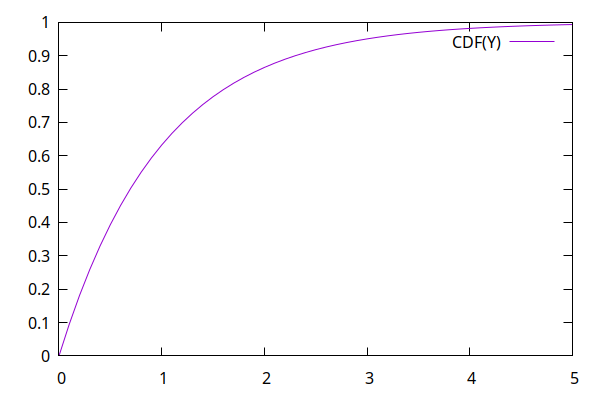
\includegraphics[width=\columnwidth]{./figs/cdf_plot.png}
    \caption{CDF of $Y$}
    \label{fig:cdf_plot}
\end{figure}


Now, we need to find $\pr{Y<1 | Y<2 }$.
For that, we need to find $F_Y(1)$ and $F_Y(2)$.\\
Using the equation for CDF,
\begin{align}
    F_Y(1) & = 1 - \frac{1}{e}
\end{align}
and
\begin{align}
    F_Y(2) & = 1 - \frac{1}{e^2}
\end{align}
Now, we can find $\pr{Y<1 | Y<2 }$ as follows,
\begin{align}
    \pr{Y<1 | Y<2 } & = \frac{\pr{Y<1 , Y<2}}{\pr{Y<2}}           \\
                    & = \frac{\pr{Y<1}}{\pr{Y<2}}                 \\
                    & = \frac{F_Y(1)}{F_Y(2)}                     \\
                    & = \frac{1 - \frac{1}{e}}{1 - \frac{1}{e^2}} \\
                    & = \frac{e(e-1)}{e^2-1}                      \\
                    & = \frac{e}{e+1}
\end{align}

\item C code to plot the cdf of $Y$.
\begin{enumerate}
\item The following code generates the data for the cdf of $Y$.
\lstdefinestyle{customc}{
  belowcaptionskip=1\baselineskip,
  breaklines=true,
  frame=L,
  xleftmargin=\parindent,
  language=C,
  showstringspaces=false,
  basicstyle=\footnotesize\ttfamily,
  keywordstyle=\bfseries\color{green!40!black},
  commentstyle=\itshape\color{purple!40!black},
  identifierstyle=\color{blue},
  stringstyle=\color{orange},
}

\lstdefinestyle{customasm}{
  belowcaptionskip=1\baselineskip,
  frame=L,
  xleftmargin=\parindent,
  language=[x86masm]Assembler,
  basicstyle=\footnotesize\ttfamily,
  commentstyle=\itshape\color{purple!40!black},
}

\lstset{escapechar=@,style=customc}
\lstset{{language=C}}
\begin{lstlisting}
        #include <stdio.h>
        #include <math.h>
        
        // Define the PDF function
        double pdf(double x) {
            if (x >= 1.0) {
                return 1.0 / (x * x);
                }
                return 0.0;
                }
                
                // Calculate the CDF of Y
                double cdf_y(double y) {
        double sum = 0.0;
        double dx = 0.0001; // Small step size for numerical integration
        double x;
        
        for (x = 1.0; x <= exp(y); x += dx) {
            sum += pdf(x) * dx;
            }
            
            return sum;
            }
            
    int main() {
        FILE *dataFile = fopen("cdf_data.txt", "w");
        
        if (!dataFile) {
            printf("Error: Could not open data file for writing.\n");
            return 1;
        }
        
        double y, cdf;
        
        // Calculate and write the CDF data
        for (y = 0.0; y <= 5.0; y += 0.1) {
            cdf = cdf_y(y);
            fprintf(dataFile, "%.2f %.5f\n", y, cdf);
            }
            
            fclose(dataFile);
            
            printf("Data file 'cdf_data.txt' generated.\n");
            
            return 0;
            }
        \end{lstlisting}
\item The following code plots the cdf of $Y$ using Gnuplot.
\lstset{{language=Gnuplot}}
\begin{lstlisting}
set terminal pngcairo enhanced color size 600,400
set output 'cdf_plot.png'
plot 'cdf_data.txt' using 1:2 with lines title 'CDF(Y)'
\end{lstlisting}
\end{enumerate}
\end{enumerate}
\end{document}
